% !TeX spellcheck = en_US
\documentclass[]{article}
\usepackage{graphicx}
\usepackage{float}
\usepackage{hyperref}

%opening
\title{VietAI ACV03 Course project on topic:	\\Cityscape Scene Semantic Understanding for Driving Assistant
}
\author{Huynh Tan Cuong}

\begin{document}

\maketitle


\section{Problem}

Considering the concept of autonomous driving, cityscape understanding at semantic level is such a challenging task to date. In this project, you propose a simple ADAS, containing a cityscape understanding system and a virtual driving instructor. To be specific, you can leverage a semantic scene understanding system to understand the cityscape, and then utilize a pre-trained LLM to give driving instruction based on the context extracted from the understanding system. Below are exemplary cases.

\begin{figure}[H]
\centering
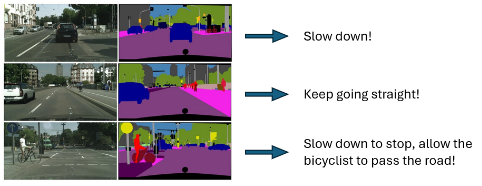
\includegraphics[width=0.7\linewidth]{problem}
\caption{Cityscape Scene Semantic Understanding}
\label{fig:problem}
\end{figure}

\section{Proposed solution}

This project implements a semantic scene understanding pipeline for autonomous driving assistance using the SegFormer model. It performs semantic segmentation on cityscape images and videos, analyzes spatial relationships between detected objects, and generates natural language scene descriptions suitable for large language models (LLMs). The system can recommend movement decisions (such as direction, speed, and hazard avoidance) based on real-time visual input.

\begin{figure}[H]
\centering
\includegraphics[width=0.9\linewidth]{demo}
\caption{Demo of solution}
\label{fig:demo}
\end{figure}

Link to repository: 
\href{https://github.com/huynhtancuong/Cityscape-Scene-Semantic-Understanding-for-Driving-Assistant}{Github Repository}

Link to presentation:
\href{https://docs.google.com/presentation/d/1laEV4_pjnoPKA--Y0ge82wpDJI7srnGeBBZ18IxpRNI/edit?usp=sharing
}{Google Slide}

Link to demo video:
\href{https://youtu.be/dK-Rmfju8zg}{Youtube Video}




\end{document}
